\chapter{Основное задание}

\section{Содержание проекта}

Группа из 7 человек, длительностью не более 3 месяцев, бюджет не более 675 тысяч рублей.

\section{Задание 1: Настройка рабочей среды проекта}

Установлена дата начала проекта: 1 апреля 2024 года~---~первый понедельник 2 квартала.

\begin{figure}[H]
    \begin{center}
    \includegraphics[width=1\linewidth]{assets/1.png}
    \caption{Установка даты начала проекта}
    \label{fig:1}
    \end{center}
\end{figure}

Установлены параметры расписания проекта: длительность работы в днях, объем работы в часах, тип работ по умолчанию~---~с фиксированными трудозатратами.

\begin{figure}[H]
    \begin{center}
    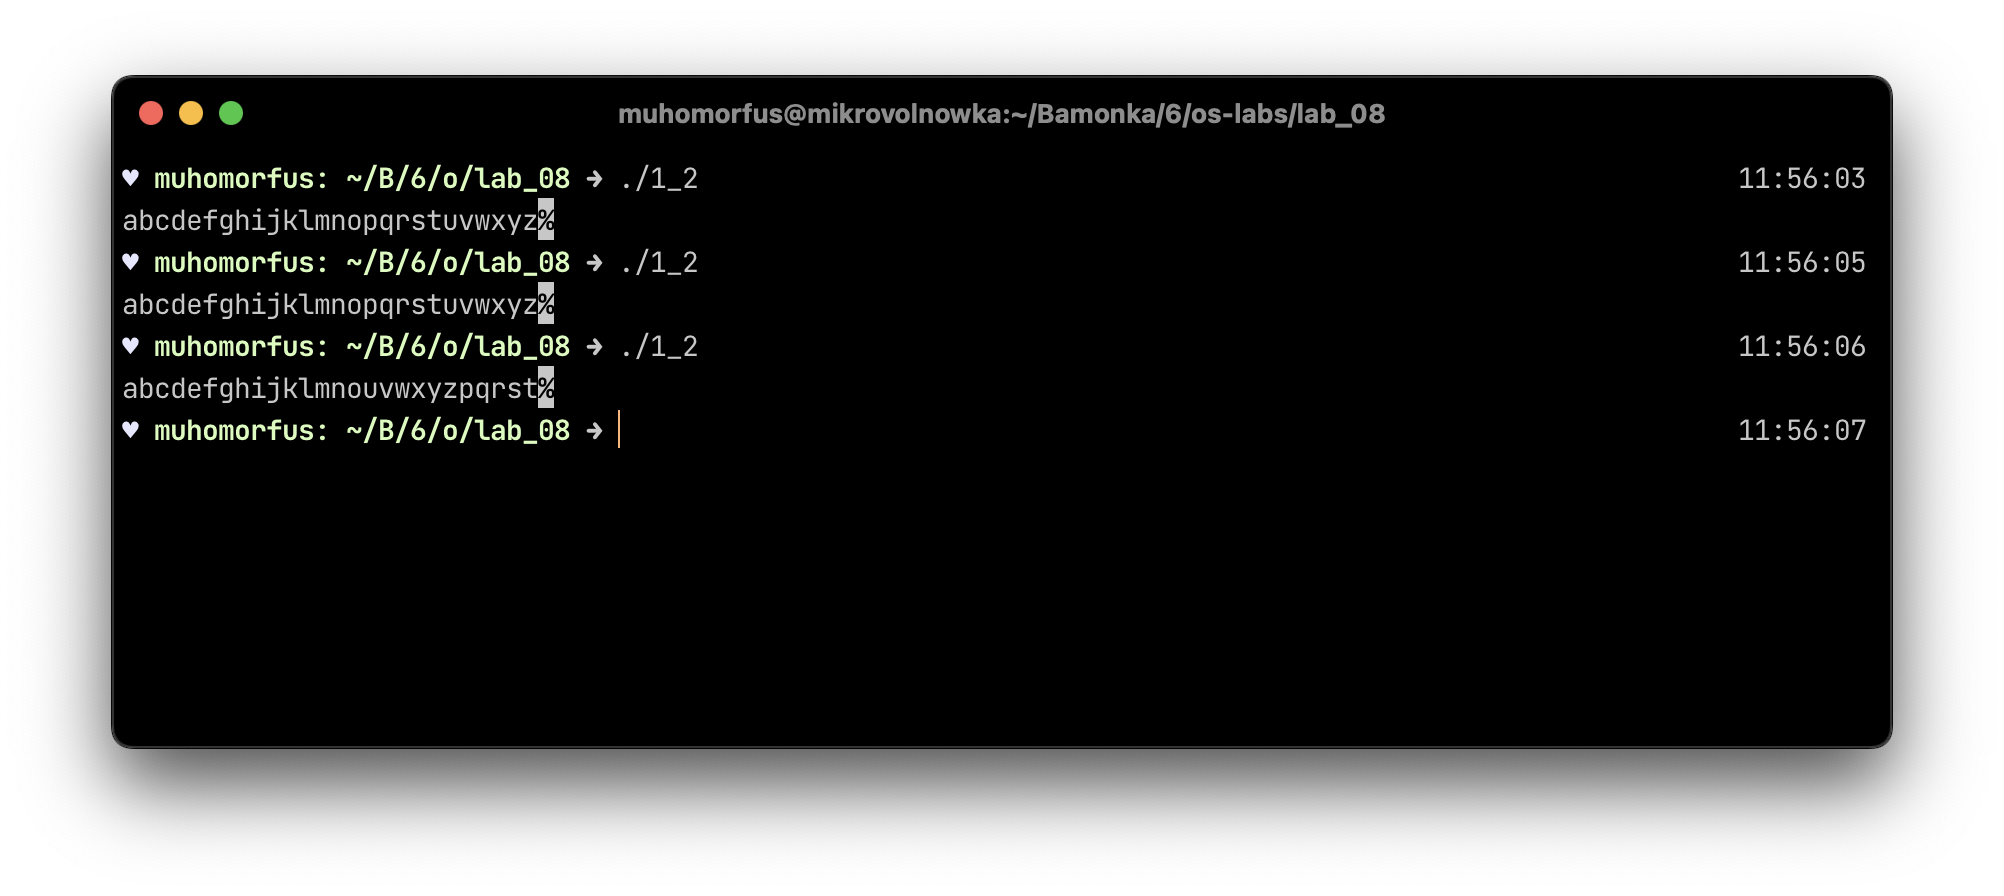
\includegraphics[width=1\linewidth]{assets/2.png}
    \caption{Установка расписания}
    \label{fig:2}
    \end{center}
\end{figure}

Установлен стандартный календарь рабочего времени и проставлены праздники.

\begin{figure}[H]
    \begin{center}
    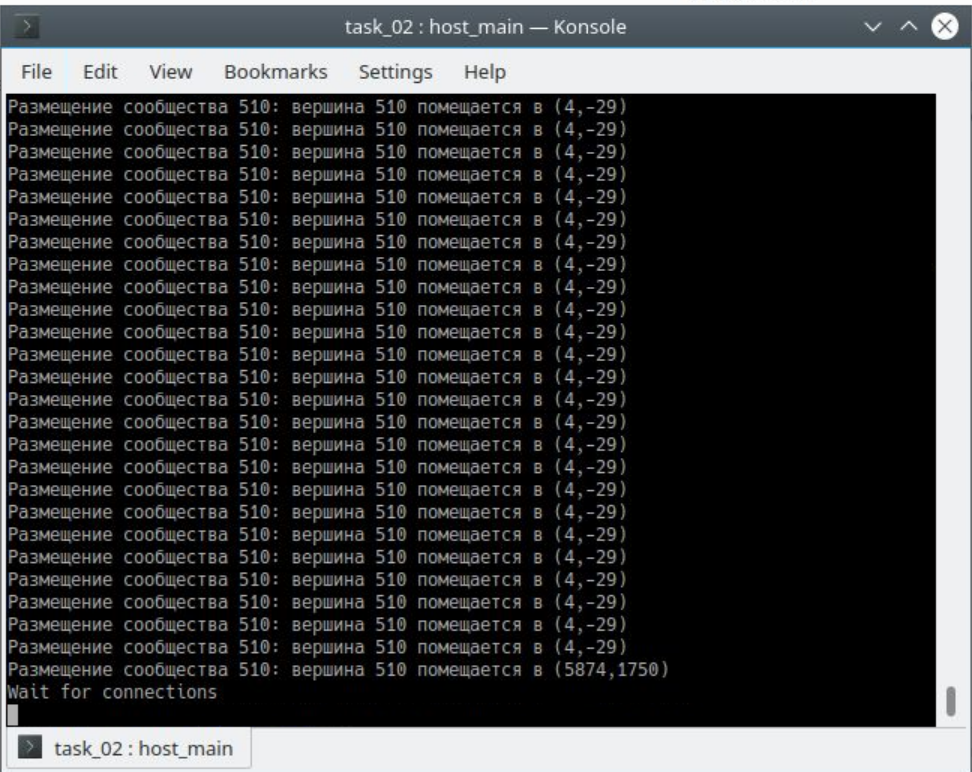
\includegraphics[width=1\linewidth]{assets/3.png}
    \caption{Установка рабочего времени}
    \label{fig:3}
    \end{center}
\end{figure}

\section{Задание 2: Создание списка задач}

Введены задачи в соответствии с заданием.

\begin{figure}[H]
    \begin{center}
    \includegraphics[width=1\linewidth]{assets/4.png}
    \caption{Созданные задачи}
    \label{fig:4}
    \end{center}
\end{figure}

\section{Задание 3: Структурирование списка задач}

Произведена группировка задач: задачи 5-6 стали подзадачами задачи 4, задачи 9-12 стали подзадачами задачи 8.

\begin{figure}[H]
    \begin{center}
    \includegraphics[width=1\linewidth]{assets/5.png}
    \caption{Сгруппированные задачи}
    \label{fig:5}
    \end{center}
\end{figure}

\section{Задание 4: Установление связей между задачами}

Были установлены связи в соответсвии с заданием. 

\begin{figure}[H]
    \begin{center}
    \includegraphics[width=1\linewidth]{assets/7.png}
    \caption{Задачи со связями}
    \label{fig:7}
    \end{center}
\end{figure}


Связи устанавливались в меню «Предшественники»:

\begin{figure}[H]
    \begin{center}
    \includegraphics[width=1\linewidth]{assets/6.png}
    \caption{Меню «Предшественники»}
    \label{fig:6}
    \end{center}
\end{figure}

\section{Задание 5: Создание списка ресурсов}

Созданы ресурсы в соответствии с заданием.

\begin{figure}[H]
    \begin{center}
    \includegraphics[width=1\linewidth]{assets/8.png}
    \caption{Лист ресурсов}
    \label{fig:8}
    \end{center}
\end{figure}

Добавлено примечание о том, что Соколов является ведущим программистом, а Петров руководителем дизайнерской группы.

\begin{figure}[H]
    \begin{center}
    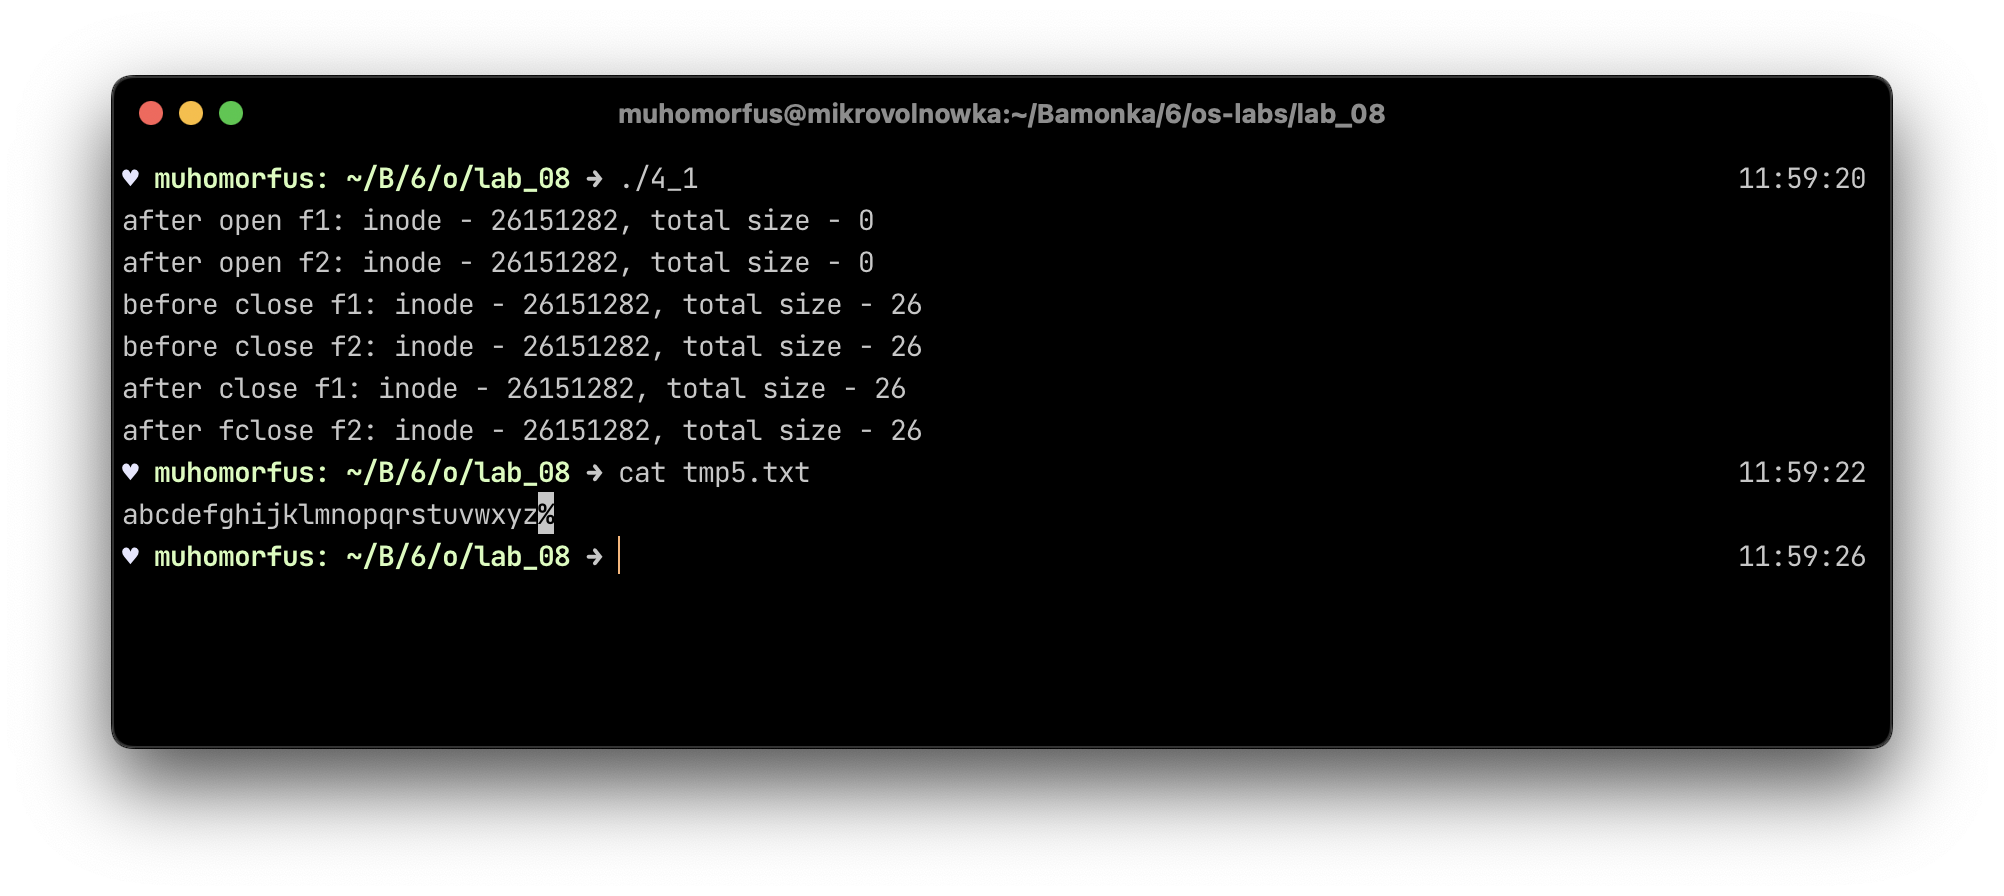
\includegraphics[width=1\linewidth]{assets/9.png}
    \caption{Заметки}
    \label{fig:9}
    \end{center}
\end{figure}

\section{Задание 6: Назначение ресурсов задачам}

Были назначены ресурсы задачам в соответствии с заданием.

\begin{figure}[H]
    \begin{center}
    \includegraphics[width=1\linewidth]{assets/10.png}
    \caption{Назначенные ресурсы}
    \label{fig:10}
    \end{center}
\end{figure}

\section{Задание 7: Оптимизация загрузки ресурсов}

Задачи по разработке представительских сайтов разбиты на 2 подзадачи: разработку дизайна (2 дня) и программирования (3 дня).

\begin{figure}[H]
    \begin{center}
    \includegraphics[width=1\linewidth]{assets/11.png}
    \caption{Разбиение задач}
    \label{fig:11}
    \end{center}
\end{figure}

В результате оптимизации стоимость проекта уменьшилась с 625850 до 600850 рублей, а дата окончания проекта не изменилась.

\section{Задание 8: Переназначение ресурсов}

Ресурс Соколов был назначен на обучение персонала.

\begin{figure}[H]
    \begin{center}
    \includegraphics[width=1\linewidth]{assets/12.png}
    \caption{После назначения Соколова на обучение персонала}
    \label{fig:12}
    \end{center}
\end{figure}

В результате у Соколова появилась перегрузка (так как он одновременно занимается установкой ПО). Сумма проекта увеличилась до 630190 рублей, а дата окончания уменьшилась до 21 июня.

Количество единиц ресурса Преподаватели сократилось до 300\%. В результате стоимость проекта уменьшилась до 617590.

\begin{figure}[H]
    \begin{center}
    \includegraphics[width=1\linewidth]{assets/13.png}
    \caption{После сокращения ресурсов Преподаватели}
    \label{fig:13}
    \end{center}
\end{figure}

Соколов был поставлен на задачу по обучению персонала после того, как он завершит работы по установке ПО.

\begin{figure}[H]
    \begin{center}
    \includegraphics[width=1\linewidth]{assets/14.png}
    \caption{Соколов сместился}
    \label{fig:14}
    \end{center}
\end{figure}

\begin{figure}[H]
    \begin{center}
    \includegraphics[width=1\linewidth]{assets/15.png}
    \caption{Результат}
    \label{fig:15}
    \end{center}
\end{figure}

В результате затраты уменьшились до 590640 рублей.

Для установки ПО у Соколова был установлен профиль нагрузки Загрузка в начале, для обучения персонала Загрузка в конце.

\begin{figure}[H]
    \begin{center}
    \includegraphics[width=1\linewidth]{assets/16.png}
    \caption{Изменение профила нагрузки}
    \label{fig:16}
    \end{center}
\end{figure}


В результате проделанных оптимизаций, стоимость проекта упала с 630190 рублей до 590640 рублей, а дата окончания проекта изменилась с 25 июня до 3 июля.

\section{Задание 9: Уточнение плана проекта}

С помощью диаграммы Ганта с отслеживанием был получен критический путь проекта.

\begin{figure}[H]
    \begin{center}
    \includegraphics[width=1\linewidth]{assets/17.png}
    \caption{Критический путь}
    \label{fig:17}
    \end{center}
\end{figure}

В рамках оптимизации были выполнены следующие изменения:

\begin{itemize}
	\item На задачу с Установкой ПО дополнительно были назначены Тимофеев, Соломин и Яковлева.
	\item Тип связи у обучения персонала с установкой ПО был изменен на ОН.
	\item На программирование сайта были назначены Соколов и Петров.
	\item На тестирование сайта были назначены Соколов, Петров и Тимофеев.
\end{itemize}

\begin{figure}[H]
    \begin{center}
    \includegraphics[width=1\linewidth]{assets/18.png}
    \caption{Результат оптимизаций}
    \label{fig:18}
    \end{center}
\end{figure}

В результате оптимизаций стоимость увеличилась с 590640 рублей до 598281 рублей. Дата окончания изменилась с 3 июля до 27 мая. Проект укладывается в бюджет и в сроки.

\section{Задание 10: Контроль за реализацией проекта}

Была установлена дата отчета 1 мая. Была внесена фактическая информация о выполнении проекта:

\begin{itemize}
	\item Установка ПО была завершена на 100\%
	\item Обучение персонала было завершено на 70\%
	\item Разработка дизайна сайта 1 была завершена на 20\%
	\item Проектирование сайта было завершено на 50\%
	\item Зарплата Яковлевой составила 100000 рублей
\end{itemize}

Линия прогресса: 

\begin{figure}[H]
    \begin{center}
    \includegraphics[width=1\linewidth]{assets/19.png}
    \caption{Результат оптимизаций}
    \label{fig:19}
    \end{center}
\end{figure}

По графику видно, что обучение персонала отстает от базового плана, а проектирование сайта и разработка дизайна сайта 1 --- опережает.

Можно проанализировать стоимостные параметры проекта по методике освоенного объема.

\begin{figure}[H]
    \begin{center}
    \includegraphics[width=1\linewidth]{assets/20.png}
    \caption{Освоенный объем}
    \label{fig:20}
    \end{center}
\end{figure}

На основании таблицы можно сделать следующие выводы.

\begin{itemize}
	\item ОКП у обучения персонала составляет -71516 рублей. Это значит, что обучение персонала отстает по времени от базового плана.
	\item ОКП у дизайна сайта 1 составляет 1000 рублей. Это значит, что задача опережает по времени базовый план.
	\item ОКП у проектирования сайта составляет 18125 рублей. Это значит, что задача опережает по времени базовый план.
	\item ОПС у установки ПО составило 10416 рублей. Это значит, что затраты больше, чем планировалось.
	\item ОПС у обучения персонала составило 29385 рублей. Это значит, что затраты больше, чем планировалось.
	\item ПОПЗ составляет 676591 рубль, ОПЗ 78309 рублей. Это значит, что проект, если не сделать оптимизации, не уложится в бюджет. Это связано с увеличением зарплаты для Яковлевой.
\end{itemize}



